\chapter{Proportional controller design}

\section{Specifying the problem}
In designing a proportional controller, the only parameter that can be improved is percent overshoot $ \% OS $. Since there is no design requirement, the problem is randomly specified as: 

\textbf{Design the value of gain, $ K_p $ to yield $ 10\% $ overshoot for a unit step input.}

\section{Solving the problem}
Since the plant is approximated as a second-order system, the damping ratio $ \zeta $ is
\begin{equation}
	\zeta = \dfrac{-\ln(\% OS)}{\sqrt{\pi^2 + \ln^2(\% OS)}} = \dfrac{-\ln(10/100)}{\sqrt{\pi^2 + \ln^2(10/100)}} = 0.591
\end{equation}

A program is written for drawing the root locus and will be shown later. The purpose is to find the intersection between the desired damping ratio and and root locus. From the figure, it is found that $ K_p = 0.9827 $ at the closed-loop poles $ s = -2.5 \pm j3.411 $. The closed-loop transfer function with unity feedback is:
\begin{equation}
		\dfrac{\Theta_L(s)}{V_f(s)} = \dfrac{17.885}{s^2 + 5s + 17.885}
\end{equation}

The natural frequency is
\begin{equation}
	\omega_n = \sqrt{17.885} = 4.23
\end{equation}

The settling time is
\begin{equation}
	T_s = \dfrac{4}{\zeta\omega_n} = \dfrac{4}{0.591\times 4.23} = 1.6
\end{equation}

The peak time is
\begin{equation}
	T_p = \dfrac{\pi}{\omega_n\sqrt{1-\zeta^2}} = \dfrac{\pi}{4.23\sqrt{1-0.591^2}} = 0.92
\end{equation}

Since the system is Type 1, the static error constant for ramp input is
\begin{equation}
	K_v = \lim\limits_{s\rightarrow 0} sK_pG(s) = \dfrac{0.9827\times 18.2}{5} = 3.577
\end{equation}
and the steady-state error is
\begin{equation}
	e_{ramp}(\infty) = \dfrac{1}{K_v} = \dfrac{1}{3.577} = 0.28
\end{equation}

For unit step input, the steady-state error is $ e_{step}(\infty) = 0 $ (type 1 system).

\section{Graphic results}
\subsection{Transfer function of the gain controller}
\begin{minted}{python}
	from control import *
	from numpy import *
	from matplotlib.pyplot import *
	
	
	G = tf(18.2, [1, 5, 0])
	rlocus(G)
	
	zeta = -log(0.1)/sqrt(pi**2 + log(0.1)**2)
	x = array([-5, 0])
	
	plot(x, tan(pi-arccos(zeta))*x)
	plot(*step_response(feedback(G, 1)))
\end{minted}

\begin{figure}[ht]
	\centering
	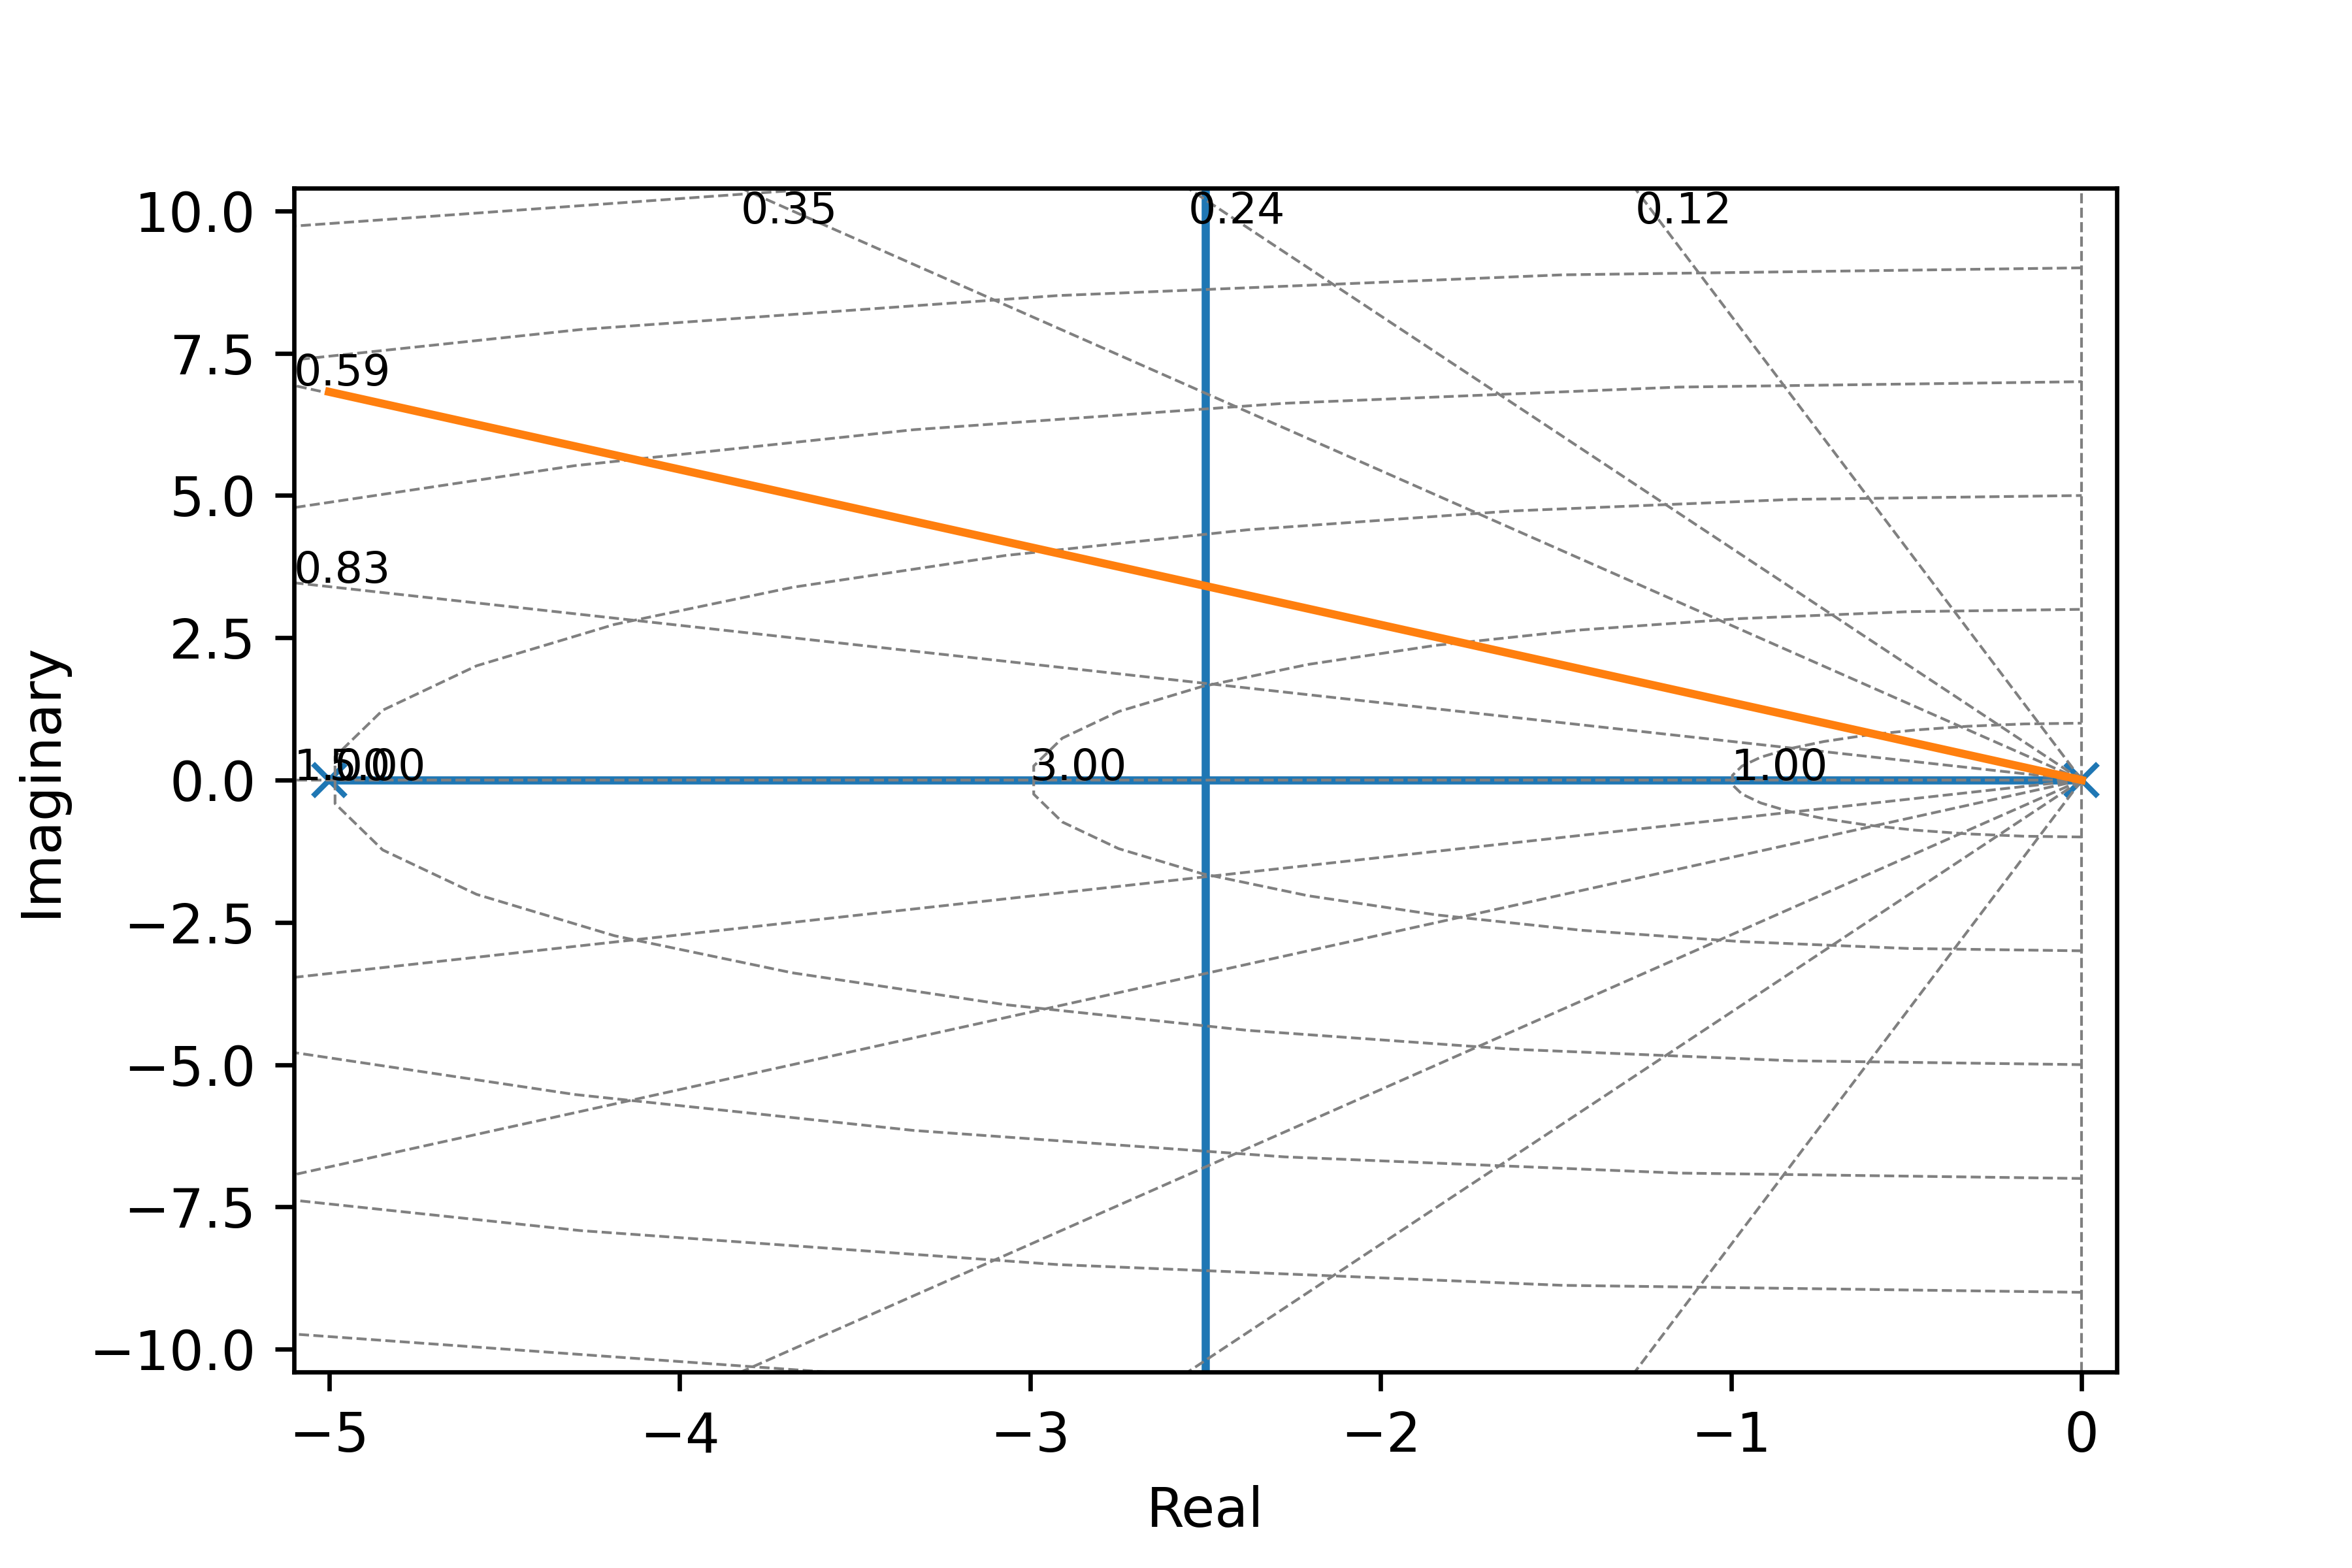
\includegraphics[width=0.7\linewidth]{rlocus}
	\caption{Root locus of the open-loop uncompensated system}
	\label{f1}
\end{figure}

\subsection{Transient response of the system}
\begin{minted}{python}
	from control import *
	from numpy import *
	from matplotlib.pyplot import *
	
	
	G = tf(18.2, [1, 5, 0])
	sys = feedback(0.9827*G, 1)
	
	plot(*step_response(sys))
\end{minted}
\begin{figure}[ht]
	\centering
	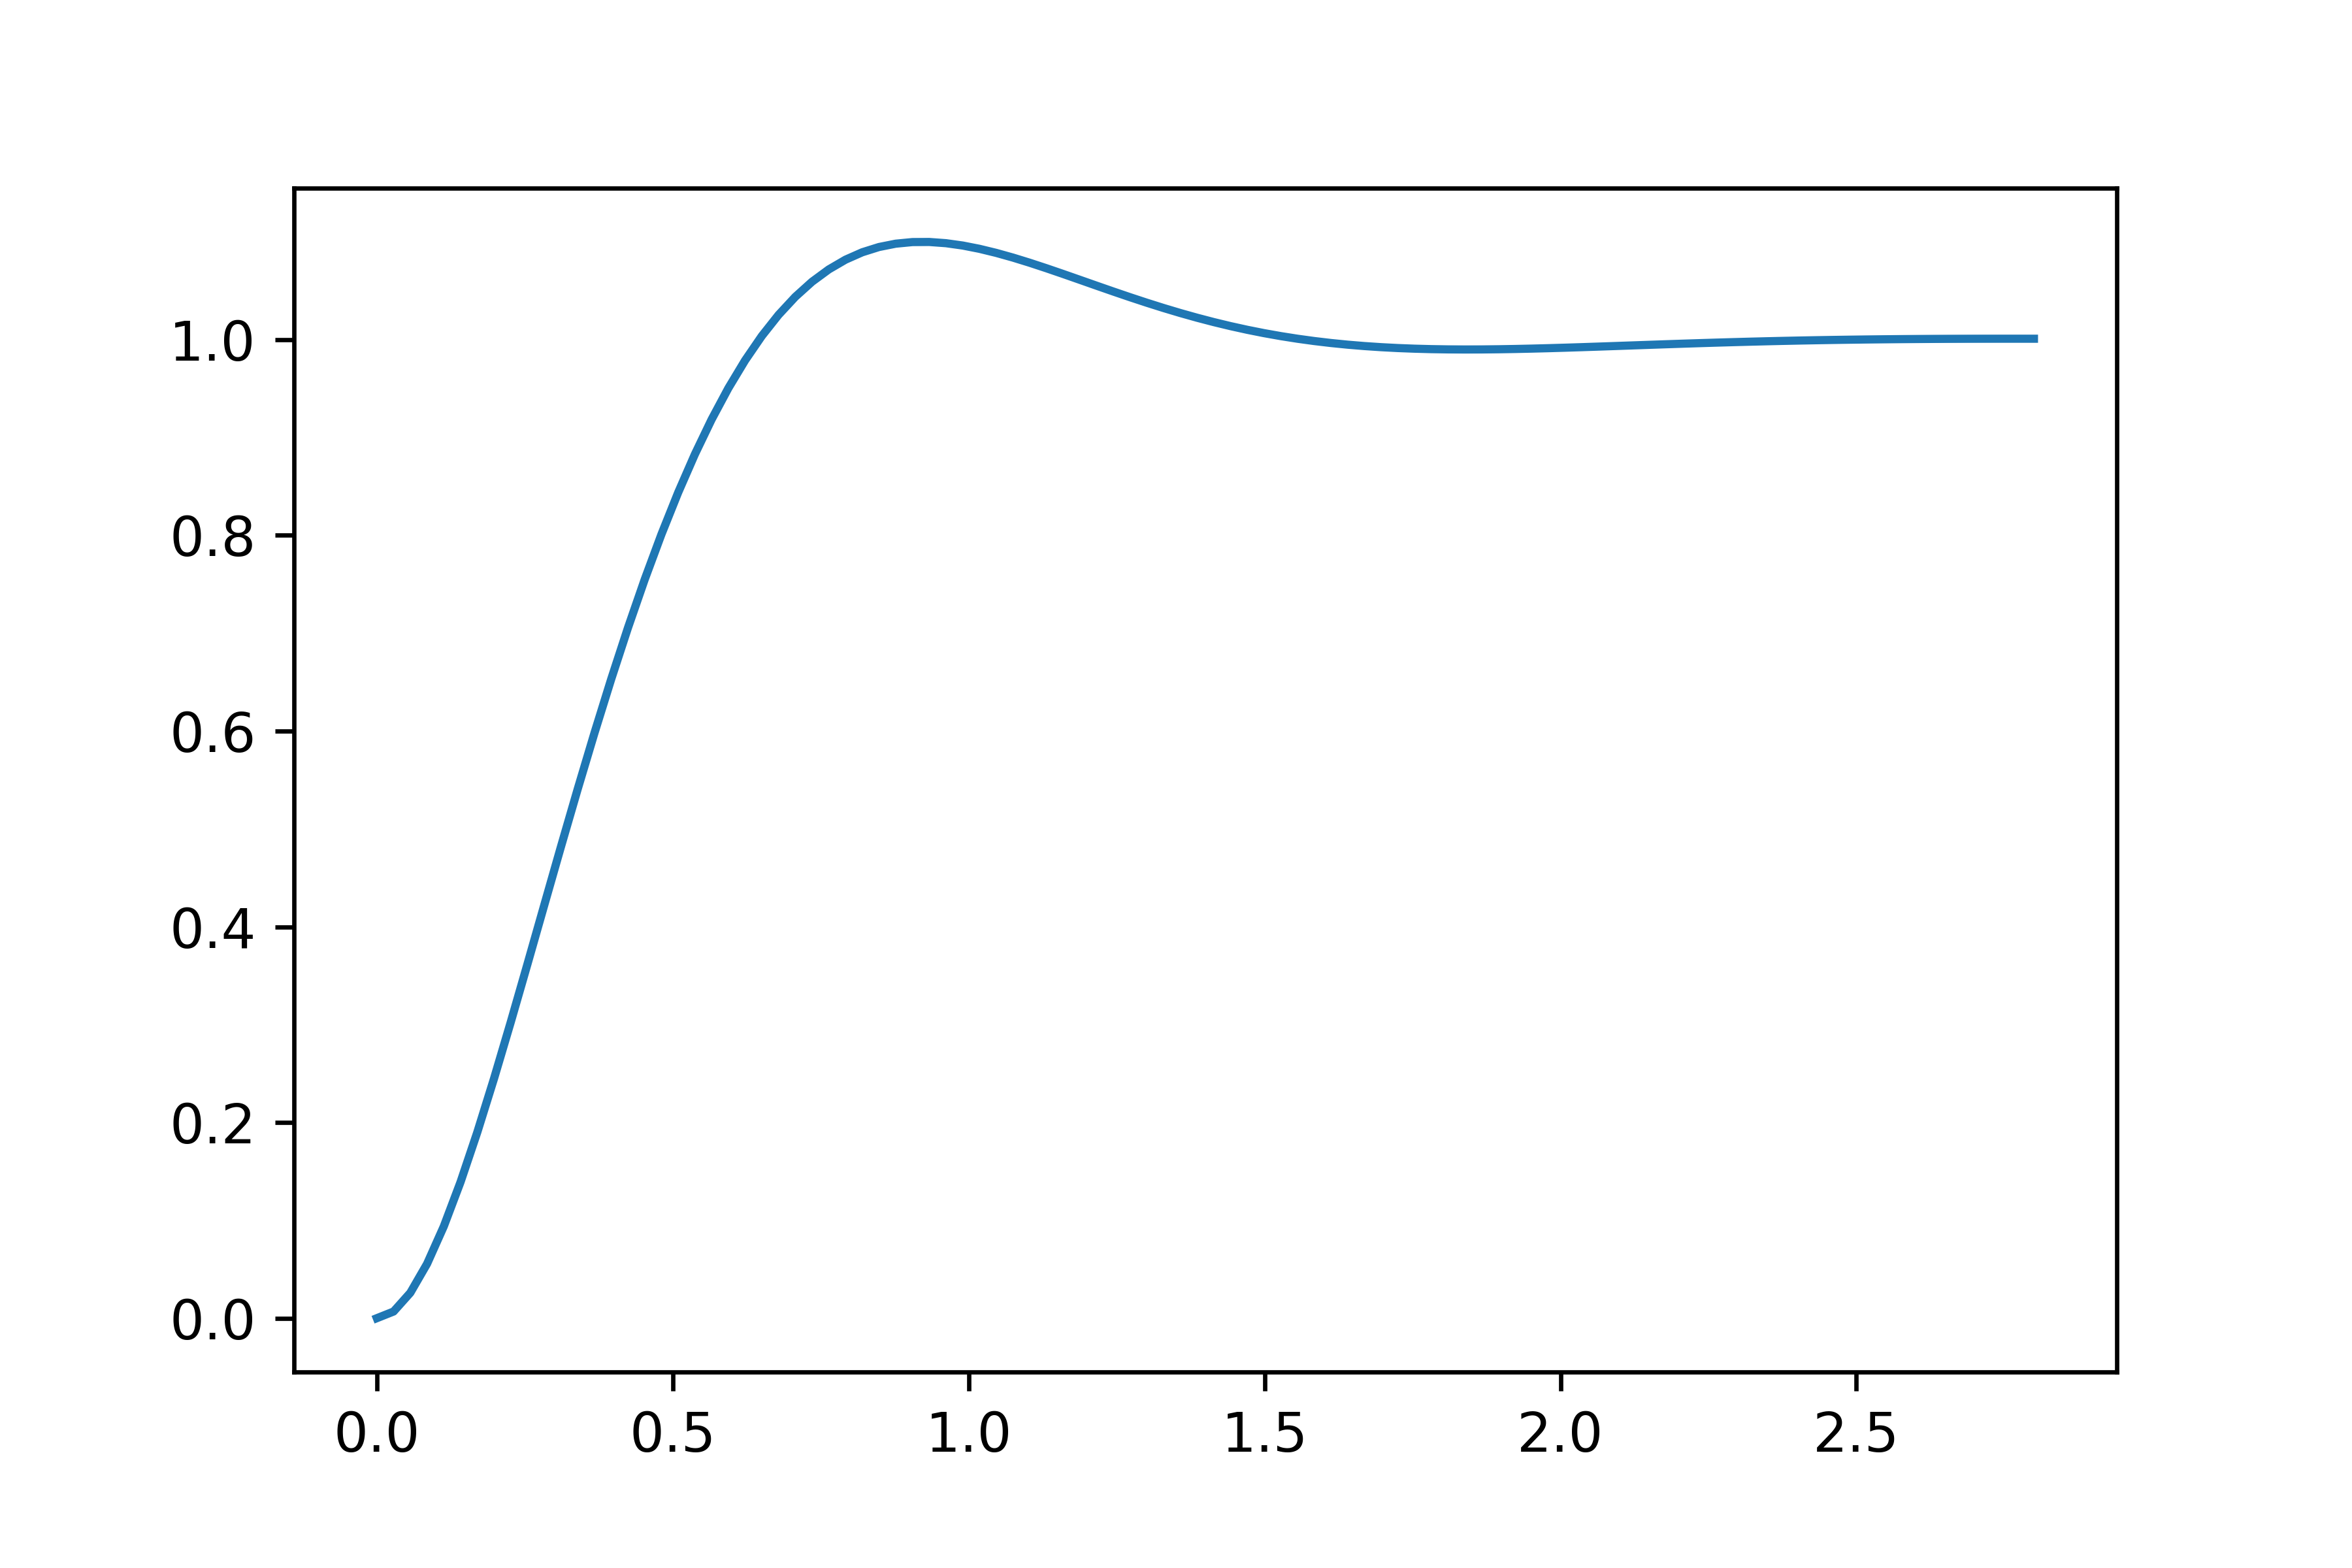
\includegraphics[width=0.7\linewidth]{stepKp}
	\caption{Step response of the system using proportional gain controller}
\end{figure}
